
\section{Experiments}

\subsection{Overview}

In this section, we describe our experimental evaluation of PC.
The aim is to answer
following questions:

\begin {enumerate}
\item PC has been designed to facilitate the construction of high-performance Big Data tools and libraries by programmer
comfortable with lower-level systems concepts, including memory management.
How useful is PC for this task?
\item PC's core design goals were ``declarative in the large,
high-performance in the small.'' The latter goal---high performance in the small---was largely realized via the 
PC object model.  We wish to answer the question: Can the PC object model be used to build 
object-oriented computations
that efficiently manipulate highly nested and complex objects?
\item Finally, machine learning (ML) is an important component of many libraries---and ML will only increase in importance
as a target for tool and library development in the future.
So we wish to ask: How well does PC compare to alternative systems for developing scalable ML algorithm implementations?
\end {enumerate}

\noindent In an attempt to answer each of these questions, we perform three different benchmarking tasks:

\begin {enumerate}
\item To test the applicability of PC for tool and library construction, we constructed a scalable, distributed
linear algebra library
called \texttt{lilLinAlg} on top of PC, and evaluated \texttt{lilLinAlg}'s performance for running three
computations that could reasonably be expressed in linear algebra: distributed Gram matrix construction, 
distributed least squares linear regression, and distributed nearest neighbor search.

\item To test the utility of the PC object model, we first denormalized the TPC-H database \cite{council2008tpc} into an object-oriented 
representation, and then benchmarked two reasonably complex 
analytical computations ---the
first computes the list of customers and the parts they construct for each supplier, and the
second is a top-$k$ similarity query that searches for the customers whose set of purchased items is most similar
to a query set.

\item Finally, we also implemented three widely used
  iterative machine learning algorithms on top of PC: Latent Dirichlet Allocation (LDA) which is used for
  textual topic mining;
  Gaussian mixture model (GMM) learning which is used to cluster data using a mixture of high-dimensional Normal
  distributions, and the simplest, $k$-means clustering (chosen because of its ubiquity as a Big Data ML benchmark).
\end {enumerate}

\vspace{5 pt}
\noindent
\textbf{Organization.}  The remainder of this section is organized as follows.  First, we describe the experimental
environment used to evaluate these implementations.  
Next we describe each of the three benchmarks, in sequence. We then conclude the experiments with a general
discussion of the results.  This includes a discussion of implementation complexity, as well as a discussion on how much
our results are (or are not) simply a direct result of coding using C++, as opposed to a managed language such as Java or
C\#.

\subsection {Experimental Environment}

All of the experiments reported in this paper were performed using a
cluster that consists of eleven Amazon EC2 \texttt{m2.4xlarge} machines,
running Ubuntu 16.04. Each machine had eight virtual cores, one SSD
disk, and 68 GB of RAM. In each PC cluster that we built, one of the eleven machines served as the master
node and the rest ten machines served as worker nodes.

Since Apache Spark is most widely-used Big Data system both for applications programming and for tool and library
development, most
(though not all) of our comparisons were with Spark (version
2.1.0). The configuration of the Spark cluster such as
executor memory, number of cores for each executor, number of
executors, data partitions and so on are carefully tuned for each
experiment. We do not clear the OS buffer cache, so HDFS data can be buffered or
cached in the OS buffer cache. For each experiment we read HDFS data
via a binary format (Parquet for the Spark Dataset API,
and a Java Object file for the Spark RDD API).  In all of the
experiments, data are serialized in Kryo format. 


\subsection {Distributed Linear Algebra}

Since PC is designed to support the construction
of high-performance tools and libraries, our first benchmarking effort was aimed at determining 
whether PC is actually useful for that task.  Thus, we asked
a PhD student (who at the outset knew nothing of PC) 
to use the system to build a small Matlab-like 
programming language and library for distributed matrix operations.
We called this implementation \texttt{lilLinAlg}.

Our goal was to determine the 
performance and functionality that an expert programmer (but PC novice) could deliver in a short
time-frame, compared to a set of established distributed Big Data linear algebra implementations:
SciDB \cite{brown2010overview, stonebraker2011architecture} (built from the ground up by a team
consisting of MIT students and professional developers over the last
nine years), Spark \texttt{mllib} \cite{meng2016mllib} 
(the Big Data matrix
implementation shipped with Spark), and SystemML \cite{boehm2014hybrid, ghoting2011systemml, boehm2016systemml}
(a matrix and machine learning implementation developed
over the last seven years by a team at IBM, built on top of Spark and Hadoop).
The student spent about six weeks in this effort.

\subsubsection{\texttt{lilLinAlg} Implementation}

In \texttt{lilLinAlg}, a distributed matrix is stored as a set of PC \texttt{Object}s, where each 
object in the set is a \texttt{MatrixBlock}, storing a contiguous rectangular sub-block of the matrix:

\begin{code}
class MatrixBlock : public Object {
private:
    MatrixMeta meta;
    MatrixData data;
};
\end{code}

\noindent where \texttt{MatrixMeta} and \texttt{MatrixData} are defined as:

\begin{code}
class MatrixMeta : public Object {
private:
    int blockRowIndex; // row index of this block
    int blockColIndex; // col index of this block
    int totalRows; // total number of rows in matrix 
    int totalCols; // total number of cols in matrix
};

class MatrixData : public Object {
private:
    Handle<Vector <double>> rawData;
    int rowNums; // number of rows in this block
    int colNums; // number of cols in this block
};
\end{code}

\noindent \texttt{MatrixMeta} stores the location of the block in the overall matrix, and
\texttt{MatrixData} stores the actual contents of the matrix.
The actual data stored in a \texttt{MatrixData} object should be small enough to fit completely in 
a PC page (by default, PC's page size is 256MB).  A typical \texttt{MatrixData} object stores a
1,000 by 1,000 sub-matrix that is eight megabytes in size.

\texttt{lilLinAlg} uses the \texttt{MatrixBlock} object to implement a set of common distributed matrix
computations, including \texttt{transpose},
\texttt{inverse}, \texttt{add}, \texttt{subtract}, \texttt{multiply}, \texttt{transposeMultiply}, 
\texttt{scaleMultiply}, \texttt{minElement},
\texttt{maxElement}, \texttt{rowSum}, \texttt{columnSum}, \texttt{duplicateRow}, \texttt{duplicateCol}, 
and many more.  However, \texttt{lilLinAlg} programmers do not call these operations directly, rather,
\texttt{lilLinAlg} implements its own Matlab-like DSL.  
Given a computation in the DSL, \texttt{lilLinAlg} first parses the computation into an abstract syntax tree (AST), and then
uses the AST to build up a graph of PC \texttt{Computation} objects which is used to implement the distributed computation.
For example, at a \texttt{multiply} node in the compiled AST, \texttt{lilLinAlg} 
will execute a PC code similar to the following:

\begin{codesmall}
Handle <Computation> query1 = makeObject <LAMultiplyJoin> ();
query1->setInput (0, leftChild->evaluate(instance));
query1->setInput (1, rightChild->evaluate(instance));
Handle <Computation> query2 = makeObject <LAMultiplyAggregate> ();
query2->setInput(query1);
\end{codesmall}

\noindent Here, \texttt{LAMultiplyJoin} and \texttt{LAMultiplyJoin} are 
both user-defined \texttt{Computation} classes that are
derived from PC's \texttt{JoinComp} class and \texttt{AggregateComp} class, respectively; these classes are chosen 
because distributed matrix multiplication
is basically a join followed by an aggregation.
Internally, the \texttt{LAMultiplyJoin}
and \texttt{LAMultiplyAggregate} invoke the Eigen numerical processing
library~\cite{eigen} to manipulate \texttt{MatrixBlock} objects.
For example, \texttt{LAMultiplyJoin} must efficiently multiply the sub-matrices stored inside of two matrix blocks.
To accomplish this, inside of the \texttt{getProjection ()} operation for
\texttt{LAMultiplyJoin} is a native C++ lambda that contains the following code:

\begin{code}
Handle<MatrixBlock> resultMatrixBlock = makeObject <MatrixBlock> (...);
Eigen::Map<Eigen::Matrix<double,Eigen::Dynamic,Eigen::Dynamic,Eigen::RowMajor>> 
   productMatrix(resultMatrixBlock->getRawDataHandle()->c_ptr(), ...);
productMatrix = currentMatrix1 * currentMatrix2;
\end{code}

\noindent This code first makes a new \texttt{MatrixBlock} object that will store the result of the multiplication.
 It then creates an 
Eigen row major matrix object whose storage is located at 
\texttt{resultMatrixBlock->}\-\texttt{getRaw}\-\texttt{DataHandle()->}\-\texttt{c\_ptr()}.  This
sequence of calls
returns a \texttt{double} pointer that references the location of the contiguous block of \texttt{double}s inside of
the \texttt{resultMatrixBlock} object.
The Eigen package then works with those raw bytes directly,
and the overloaded \texttt{*} operator will write its result to that location.

\texttt{lilLinAlg}'s DSL looks a lot like Matlab and allows very short and easy-to-read codes.
For example, 
a least squares linear regression over a large input matrix can be easily coded as

\begin{code}
X = load(myMatrix.data); 
y = load(myResponses.data); 
beta = (X '* X)^-1 %*% (X '* y)
\end{code}

\noindent In the above DSL expression, \texttt{'*} represents a transpose-then-multiply computation,
\texttt{\^{}-1} represents an inverse computation, and \texttt{ \%*\%}
represents a multiply computation. 

\subsubsection {Experiments}

Our experimental benchmark consisted of three different computations:
a Gram matrix computation (given a matrix $\textbf{X}$, compute
$\textbf{X}^T \textbf{X}$), least squares linear regression (given a matrix of features $\textbf{X}$ and
responses $\textbf{y}$, compute 
$\hat{\pmb{\beta}} = (\textbf{X}^{T} \textbf{X})^{-1} \textbf{X}^{T} \textbf{y}$), and nearest
neighbor search in a Riemannian metric space \cite{lebanon2006metric} encoded by matrix $\textbf{A}$ (that is,
given a query vector
$\textbf{x}'$ and matrix $\textbf{X}$, find the $i$-th row in the matrix that minimizes 
$d_{\textbf{A}}^2(\textbf{x}_i, \textbf{x}') = 
(\textbf{x}_i - \textbf{x}')^T\textbf{A}(\textbf{x}_i - \textbf{x}')$).  
For each computation we used three different data dimensionalities: ten, $10^2$, and $10^3$.  This refers to
the number of features or entries in each data point. 
For
all three computations, 
$10^6$ data points were used. 

In addition to \texttt{lilLinAlg}, 
for the Gram matrix and linear regression computations, SystemML V0.9 on Hadoop was used.
For these two computations, Spark \texttt{mllib} along with
Spark 1.6.1 was used.  For
nearest neighbor, SystemML V1.0 on Spark 2.1.0 was used, and for
nearest neighbor, \texttt{mllib} along with Spark 2.1.0 was used. We
use the same SciDB version---14.8---for all three
experiments.

We spent considerable effort tuning all of the implementations.
For \texttt{lilLinAlg}, this consisted mainly of efforts to choose the correct page size for holding the
\texttt{MatrixBlock} objects.  The task was balancing the ability to fully distribute the computations
(which requires a large number of small \texttt{MatrixBlock} objects) versus making sure that the computations
themselves were efficient (which requires large \texttt{MatrixBlock} objects).  We settled on 
a four MB page size for ten dimensions, a 16 MB page
size for $10^2$ dimensions, and a 64 MB page size for $10^3$ dimensions. 
PC's query optimizer dynamically decided to use a
broadcast join to implement matrix operations when one input to the join is smaller than 
two
gigabytes.  Otherwise, it uses a full hash partition join.

For the runs on the other three platforms, we also carefully tuned the
systems for best performance. For example, we tuned Spark block size and repartition
size for every experiment. In SystemML, we also carefully chose to
use the parallel for loop, which boosted performance significantly.

For fairness, for each of the distributed linear algebra tools, 
we do not count the time required to load data from client into the system
(for example, 
for \texttt{lilLinAlg}, we do not count the time required to load data from text and into PC).

\subsubsection {Results and Discussion}

Experimental results are given in 
Table \ref{fig:LR}. 
This table shows that for every one of the higher-dimensional computations, the 
\texttt{lilLinAlg} implementation was the fastest.  Often, it was considerably faster.
Looking only at the nearest neighbor computation (where the latest version of Spark was used
along with Spark's \texttt{mllib}) \texttt{lilLinAlg} was five times faster than \texttt{mllib}
and thirteen times faster than SciDB.  

For the smallest, ten-dimensional computations, there was some variability in the results.
For two of the three computations, 
SystemML was the fastest.  However, in all three of the ten-dimensional computations, SystemML chose
\emph{not} to distribute the underlying computation, as it was small enough to be efficiently extracted
on a single machine.  This demonstrates that for a small computation, the overhead of performing it in 
distributed fashion across multiple machines calls into question the viability of distribution in the first place.

\begin{table}[h!]
\begin{center}
\begin{tabular}{|c||c|c|c||c|c|c||c|c|c||}
\hline
& \multicolumn{3}{c||}{Gram Matrix} & \multicolumn{3}{c||}{Linear Regression} & \multicolumn{3}{c||}{Nearest Neighbor} \\
\hline
Dimensionality & $10$ & $100$ & $1000$& $10$ & $100$ & $1000$& $10$ & $100$ & $1000$ \\
\hline
\hline
PC (\texttt{lilLinAlg}) &00:07 & 00:09 &00:39 &00:14 &00:22 &00:49& 00:15 & 00:20 & 01:06 \\
SystemML &00:05$*$ &00:51 &02:34 &00:06$*$ &00:53 &02:38 &00:04$*$ &00:30 &01:32 \\
Spark \texttt{mllib} &00:20  &00:54 &17:31 &00:35 &01:01 &17:42 &01:20 & 04:49 &14:30 \\
SciDB   &00:03 &00:17 &03:20 &00:15 &00:33 &06:04 &00:28 &02:56 & 06:24 \\
\hline
\end{tabular}
\caption{Linear algebra benchmark. Format is MM:SS.
A star ($*$) indicates running in local mode.}
\label{fig:LR}
\end{center}
\end{table}

We feel that overall, these results largely validate the hypothesis that PC is an excellent platform for the 
construction of Big Data tools and libraries.  The only distributed linear algebra implementation
to approach \texttt{lilLinAlg}s performance on the larger matrices
was SystemML.  The newest SystemML version, on Spark, is only 50\% slower than \texttt{lilLinAlg} for nearest neighbor search.
However,
SystemML was built over many years by a team of PhDs, and research papers have been written about the
technology developed for the system, including one awarded a VLDB best paper award \cite{boehm2016systemml}.
\texttt{lilLinAlg} was developed in six weeks by a single PhD student, and it is still
faster (though to be fair, SystemML has a much broader
set of capabilities than \texttt{lilLinAlg}).
One may conjecture that had SystemML been built on a platform such as PC rather than on Spark, it might be significantly
faster than it is now.

Despite the demonstrated benefits of building \texttt{lilLinAlg} on top of PC, we point out that
PC is a young system and so it is still missing some key functionality that would boost
\texttt{lilLinAlg}'s performance even more.  For example, PC cannot make use of pre-partitioning of the data stored in a set. 
If the
\texttt{MatrixBlock} objects making up a distributed
matrix could be pre-partitioned based upon the row/column at load time, it 
would mean that the expensive join for an operation
such a multiply could completely avoid a runtime partitioning of the data, which requires shuffling each input matrix.
Thus, it is not unreasonable to suggest that as PC matures, it will be even faster.

\subsection{Big Object-Oriented Data}

Programming with objects is attractive as a programming paradigm, but (as we have argued in this paper)
often costly in terms of performance, particularly
for distributed computing.  One answer is to simply disallow complex objects.  The 
developers of Apache Spark, for example, have attempted to move away from object programming
and towards a relational model of programming (with Datasets and Dataframes) 

Our solution is to allow objects, but to move away from allowing a managed environment to control 
issues such as allocation, deallocation, and data placement.  This is the approach taken in the design and implementation
of the PC object model.  Thus, the question we address in this particular set of experiments is: can the PC 
object model facilitate efficient computations of heavily nested, complex objects?

\subsubsection{Data Representation}

To do this, we implement two different complex object computations on top of PC and on top of Spark.
Both of these computations are over large datasets that store an instance of the TPC-H database \cite{council2008tpc}.
But rather than storing the dataset relationally, we denormalized the data into a set of nested objects. 
The simplest objects used in the denormalized TPC-H schema are 
\texttt{Part} objects, which do not look very different from the records in the  \texttt{part} schema of the TPC-H database.
In PC, these are defined as:

\begin{codesmall}
class Part : public Object {
private:
   int partID;
   String name;
   String mfgr;
   /* six more members... */};
\end{codesmall}

\noindent
\texttt{Supplier} objects are defined similarly.
\texttt{Lineitem} objects contain nested \texttt{Part} and \texttt{Supplier} objects:

\begin{codesmall}
class Lineitem : public Object {
private:
   Supplier supplier;
   Part part;
   int orderKey;
   int lineNumber;
   /* twelve more members... */}; 
\end{codesmall}
 
\noindent Then,
\texttt{Order} objects have a nested list of \texttt{Lineitem} objects, and \texttt{Customer} objects have a nested
list of all of the
\texttt{Lineitem} objects for a given customer:

\begin{codesmall}
class Order : public Object {
   Vector <Handle <LineItem>> lineItems;
   int orderkey;
   int custkey;
   /* seven more members... */};

class Customer : public Object {
   Vector <Handle <Order>> orders;
   int custkey;
   String name;
   /* seven more members... */};
\end{codesmall}

\subsubsection{Implementation and Experiments}
We then run two computations over the resulting set of \texttt{Customer} objects.  
The first computation is the \emph{parts per supplier per customer} computation where we
compute, for each supplier,
the complete list of \texttt{partkey}s that the supplier has sold to each of the supplier's customer's.
For each supplier, the result is a an object that contains the supplier's name (as a \texttt{String}) and
an object of type \texttt{Map <String, Handle <Vector <int}\texttt{>}\texttt{>}\texttt{>}.  In this
object, the \texttt{String} is the name of the customer, and the \texttt{Vector} stores the list of
\texttt{partkey}s sold to that customer.

To run this computation on PC, we use two different PC \texttt{Computation} classes.  The first, 
\texttt{Customer}\-\texttt{MultiSelection}, transforms each 
\texttt{Customer} object to one or more
\texttt{SupplierInfo} objects. Each \texttt{SupplierInfo} contains
the name of a supplier
and a \texttt{Handle} to a \texttt{Map} whose key is the name of the customer and whose value is the list
of \texttt{partkey}s that the supplier has sold to the customer.
The second \texttt{Computation}, called
\texttt{CustomerSupplierPartGroupBy},
groups all of those \texttt{SupplierInfo} objects according to the name of the supplier, computing, for each
supplier, the map from customer name to \texttt{Vector} of \texttt{partkey}s.

On Spark we implemented an algorithmically equivalent
carefully-tuned code that in the
end was not dis-similar from the PC
version.  We used
Spark version
2.1.0.
Note that since the objects are all highly nested, it was not possible to develop a satisfactory
Dataset or Dataframe implementation, and so our Spark implementation made use of Spark's RDD interface.  All
implementation was done in Java.  Since Spark makes use of lazy evaluation, it is not possible to collect a timing
for this computation unless we actually \emph{do} something with the result.  So in both the PC and the Spark computations
we add a final count of the number of customers in each \texttt{Map} in each \texttt{SupplierInfo} object.

The second computation run over the denormalizd TPC-H schema is the \emph{top-k closest customer part sets} computation.
In this computation, 
for a given
\texttt{Customer} object, we go through all of the associated 
\texttt{Order} objects and obtain the complete list of
\texttt{partid}s for each order.  All duplicate \texttt{partid}s are
removed from this list, and then the Jaccard similarity between the resulting \texttt{partid} list and a special, query
list are computed.  This is done for all of the \texttt{Customer} objects, and the $k$ \texttt{partid} lists with the 
closest similarity to the query list are returned.
In PC,
the result of the computation is a list of $k$ objects containing the Jaccard similarity, the integral \texttt{custkey}, and
a \texttt{Vector <int>} that stores the complete list of unique \texttt{partid}s sold to that customer.
In PC, the C++ code required to drive this computation is as follows:
\begin{code}
Handle<Vector<int>> listOfPartIDs = 
    makeObject<Vector<int>>(199, 22, 34, 567, 1200, 37, 46, 459);
Handle<Computation> myReader = 
    makeObject<ObjectReader<Customer>>("TPCH_db", "tpch_bench_set1");
Handle<Computation> myTopK = makeObject<TopJaccard>(k, *listOfPartIDs);
myTopK->setInput(myReader);
Handle<Computation> myWriter = makeObject<Writer
    <TopKQueue<double, Handle<AllParts>>>>("TPCH_db", "result");
myWriter->setInput(myTopK);
pcContext.executeComputations (myWriter);
\end{code}

\noindent The one query-specific \texttt{Computation} object that was implemented for the top-$k$ 
closest customer part sets computation is the \texttt{TopJaccard} class, which
is responsible for extracting a value to drive the top-$k$ computation (in this case, the Jaccard similarity) as well
as the object to be associated with that value (in this case, the \texttt{custkey} and the list of 
\texttt{partid}s sold to that customer).

For both PC and for Spark, and for both computations, we created 
TPC-H dataset of various sizes: 2.4 million,
4.8 million, 9.6 million, 14.4 million, 19.2 million and 24 million
\texttt{Customer} Objects respectively.  For the ``top-$k$
closest customer part sets'' computation, $k$ was chosen to be $\frac{1024}{2.4 \times 10^6}$ times the size
of the data.

For both Spark computations, we performed two runs at each dataset size.
For the first, we stored the data in HDFS, and measure the time to execute the query starting with a
read from HDFS.
For the second, we made sure that the data were de-serialized and stored in RAM by Spark.
To do this, we applied a \texttt{distinct().count()} operation to
an RDD storing \texttt{Customer} objects (thus ensuring full deserialization) before running each query.
All data were
serialized using Kryo, and parameters such as data partition size and parallelism are fully tuned to obtain
optimal performance. 

For PC, we run only one version of the computation, where the various \texttt{Customer} objects are stored in
PC's storage system.  Since all datasets are small enough to be cached in RAM, there is no I/O time to
retrieve data.

\subsubsection{Results and Discussion}

\begin{table}[h!]
\begin{center}
\begin{tabular}{|c||c|c|c|c|c|c|}
\hline
Number \texttt{Customer} objects &2.4M & 4.8M & 9.6M  & 14.4M & 19.2M & 24M \\
Kryo data size &41.5GB & 83.1GB & 167.2GB &251.1GB &333.2 &416.2GB \\
\hline
& \multicolumn{6}{c|}{\texttt{Customer}s per \texttt{Supplier}} \\
\hline
PlinyCompute: hot storage & 00:11&	00:19&	00:35&	00:51&	01:08&	01:21 \\
Spark: hot HDFS & 01:04&	01:53&	03:24&	04:54&	06:25&	08:16\\
Spark: in-RAM deserialized RDD & 00:16& 	00:29& 	00:56& 	01:21& 	02:18& 	03:56\\
\hline
& \multicolumn{6}{c|}{top-$k$ Jaccard} \\
\hline
PlinyCompute: hot storage & 00:03&	00:03&	00:04&	00:05&	00:05&	00:06 \\
Spark: hot HDFS & 00:56&	01:38&	03:01 & 04:01&	05:22&	06:34\\
Spark: in-RAM deserialized RDD & 00:08& 	00:12& 	00:21 & 00:32& 	01:11& 	02:38\\
\hline
\end{tabular}
\caption{PlinyCompute vs. Spark for large-scale OO computation. Times in MM:SS.}
\label{fig:TPC}
\end{center}
\end{table}

Results are in Table \ref{fig:TPC}.  The difference in speed between the PC implementation and the Spark implementation
is significant.
When Spark data
are stored in
a hot HDFS, the two computations are $6\times$ to $66\times$ faster in PC.  
This is an apples-to-apples comparison, because in both systems, the data are being fetched from system storage, where they
can be buffered in OS buffer cache or PC buffer pool respectively.

If the Spark data are already
fully deserialized and stored as an RDD in memory, then PC is still 
between $1.5\times$ and $26\times$ faster
for both computations. Since in PC there is no distinction between
serialized and deserialized data, there is no analogous case in PC. 

%While this
%may be representative of certain Spark use cases---when the same RDD is repeatedly used for querying---there are a lot of
%hidden costs that are not reflected in this time.  For example, those in-RAM RDDs may need to be garbage collected at a later
%time if a different data set is deserialized into RAM.  That cost is not included in the running times reported here.}

One of the most striking---and surprising---results was that Spark had about the same performance for both computations.  This is
a bit surprising because the top-$k$ computation seems, on the face of it, much easier 
than the ``parts per supplier per customer'' computation.  $k$ was between 1,024 and 10,240, so (in theory) that should be
a hard limit on the number of customer's whose data are moved off of each machine during a shuffle 
(since it is impossible for more than $k$
customers processed on any machine to be in the top $k$).  One explanation could be not that Spark is surprisingly slow on the
top-$k$, but that PC is relatively slow on the ``parts per supplier per customer'' computation.  Profiling reveals that PC spends
a lot of time on \texttt{String} operations (looking up particular customers in the
\texttt{Map <String, Handle <Vector <int}\texttt{>}\texttt{>}\texttt{>}, for example).  
Because PC \texttt{String}s have the same representation in-RAM and on-disk, they are purposely designed to take little
space---they do not cache hash values, for example (unlike Java \texttt{Strings}).  This might explain why PC's speedup is
less significant on that computation.

\subsection {Machine Learning}

Finally, we consider three common machine learning algorithms: LDA,
GMM and $k$-means. 

\subsubsection {Implementations}

\noindent
\textbf{Latent Dirichlet Allocation.}
The first algorithm we implemented was a Gibbs sampler for
Latent Dirichlet Allocation, or LDA.  LDA is a common text mining algorithm.
While LDA implementations are common, we
chose a particularly challenging form of LDA learning:
a 
word-based,
non-collapsed Gibbs sampler \cite{jermaineExperimental}.  The LDA implementation
is \emph{non-collapsed} because it does not integrate out the word-probability-per-topic
and topic-probability-per-document random variables. In general, collapsed implementations
that do integrate out these values are more common, but such collapsed implementations
cannot be made ergodic in a distributed setting
(where ergodicity implies theoretical correctness in some sense).
Our implementation is
\emph{word based} because the fundamental data objects it operates over are \texttt{(docID, wordID, count)} 
triples.  This generally results in a more challenging
implementation from the platform's point-of-view because it requires a many-to-one join between words
and the topic-probability-per-document vectors.  In our experiments, there are approximately
700 million such triples, and each vector is around 1KB.  Hence, the many-to-one join between them results in
700GB of data.  If the platform does not manage this carefully, performance will suffer.

The full PC LDA implementation requires fifteen different \texttt{Computation} object, as shown in 
in Figure~\ref{fig:lda-query-graph}.  Each iteration requires a 
three-way \texttt{JoinComp}, three \texttt{MultiSelectionComp}s, and three
\texttt{AggregateComp}s, among others. 

Our PC LDA computation makes use of the GSL library~\cite{gsl} to perform all necessary random sampling (non-collapsed LDA requires 
sampling from both Multinomial and Dirichlet distributions).

\begin{figure}
\centering
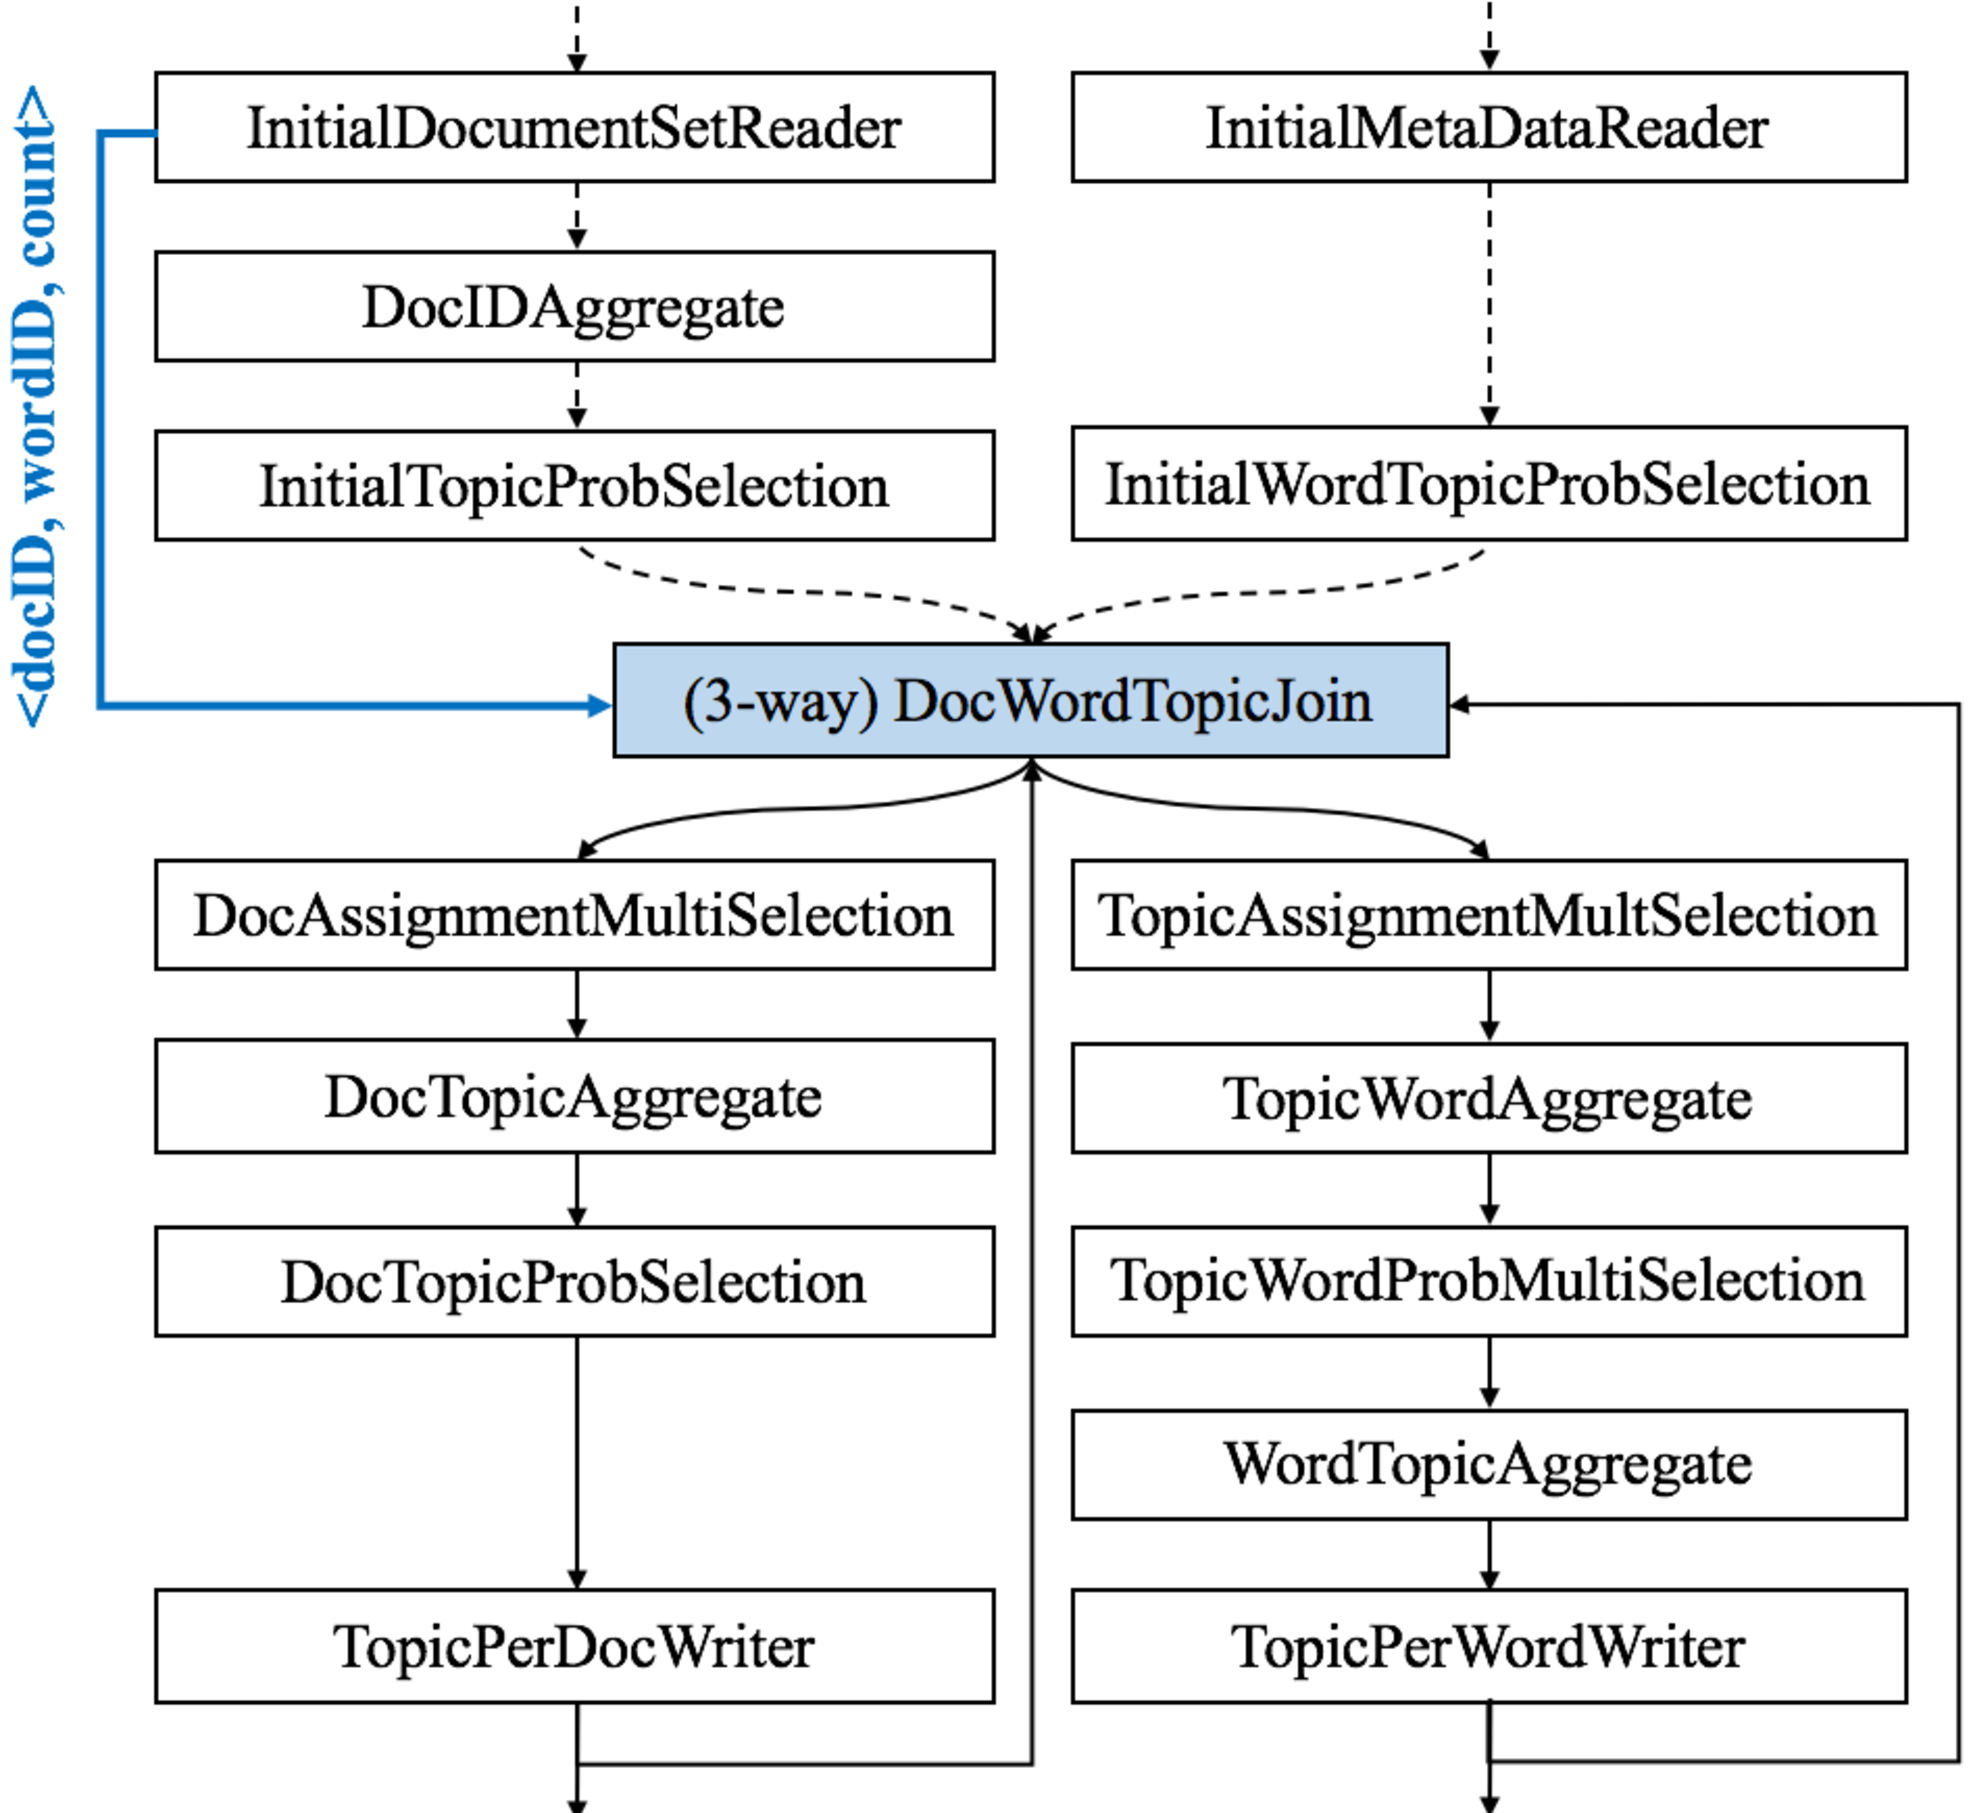
\includegraphics[width=0.5\textwidth]{lda-query-graph.pdf}
  \caption{\label{fig:lda-query-graph} PC LDA's \texttt{Computation} objects and input-output dependencies. Computations
    connected by dash lines will only run once, during  
    initialization. Computations connected by solid lines will run iteratively.}
\end{figure}

We wished to compared out LDA implementation with an algorithmically equivalent Spark implementation.  Unfortunately,
Spark \texttt{mllib}'s LDA implementation is based on expectation
maximization and online variational Bayes.
Therefore, we had a Spark expert 
carefully implement an algorithmically
equivalent word-based, non-collapsed LDA Gibbs sampler on top of Spark.  His implementation used both
Spark's RDD and Dataset        
APIs as appropriate.
The required statistical computations use the
\texttt{breeze} package. 


\vspace{5pt}
\noindent
\textbf{Gaussian Mixture Model.} A Gaussian mixture model (GMM) is a generative, statistical model where a dataset are modeled
as having been produced by a set of Gaussians (multi-dimensional Normal distributions). Learning a GMM using
the expectation maximization (EM) algorithm is one of the classical ML algorithms.
EM is particularly interesting for a distributed benchmark because in theory, the running time should be dominated
by linear algebra operations (such as repeated vector-matrix multiplications).

All linear algebra in our EM-on-PC implementation was performed using
the GSL library~\cite{gsl}.  
Our PC implementation uses a single \texttt{AggregateComp} object, which contains inside of it the current
version of the learned GMM model.  As this  \texttt{AggregateComp} is executed, a soft assignment of each
data point to each Gaussian is performed, and based off of this assignment, updates to each of the Gaussians
are accumulated.  The result of the aggregation is sent back to the \texttt{main} program where the actual update
to the model happens; the result is broadcasted in a new \texttt{AggregateComp} object, and the process begins again.

It turns out that an algorithmically equivalent implementation exists in Spark \texttt{mllib}.
Both implementations even use the same random initialization algorithm.
There are only slight differences between the two; for example, PC computes uses the standard ``log space'' trick to
compute the soft assignment and avoid underflow, whereas \texttt{mllib} uses thresholding.  

\vspace{5pt}
\noindent
\textbf{$k$-Means.} Our final ML benchmark algorithm is $k$-means.  
While not a particularly interesting computation, it is a now-classic
benchmark for Big Data ML.  We specifically developed our PC $k$-means implementation to closely match
the implementation in Spark's \texttt{mllib}.
Both implementations use the standard trick, where, to find the centroid closest to a given point,
a lower bound $||a - b||_2 \geq  abs(||a||_2 - ||b||_2)$ is
first computed to avoid unnecessary distance computations. 

\subsubsection {Experiments}

On the aforementioned eleven-node cluster, 
we ran all ML experiments using PC and Spark 2.1.0.

For LDA,  we
created a semi-synthetic document database with 2.5 million documents from
20 Newsgroups dataset by concatenating random pairs of newsgroup postings
end-on-end. There are more than 739
million \texttt{(docID, wordID, count)} triples in the dataset.
We use a dictionary size
of 20,000 words and a model size of 100 topics. 

For GMM, we generated
random data for three test cases: $10^7$ data
points with 100 dimensions, and $10^6$ data points with 300 and 500
dimensions, respectively. For each test case, the same random data was used
for comparing PC and Spark performance. For $k$-means, we
generate random data for $10^9$ data
points with ten dimensions, $10^8$ data points with 100 dimensions,  and $10^7$
data points with 1000
dimensions. Again, the same data is used on both PC and
Spark platforms.
Ten Gaussians are used for GMM, and ten clusters for $k$-means.

For each experiment, we carefully tune Spark
partition size, executor heap size and the number of cores to obtain maximum performance.
Input data for Spark are serialized
using Kryo, and read through a binary format (Parquet for the Dataset API,
and an Object file for the RDD API).

\subsubsection {Results and Discussion}

LDA Results (per iteration) are illustrated in Table~\ref{fig:LDA}.

\begin{table}[h!]
\begin{center}
\begin{tabular}{|c||c|c|c|c|c|c|}
\hline
PlinyCompute & \makecell{Spark 1: \\vanilla} & \makecell{Spark 2: also with \\join hint} & \makecell{Spark 3: also with \\forced persist} & \makecell{Spark 3: also hand-\\coded multinomial} \\
\hline
02:05 & 50:20 & 17:30 & 09:26 & 05:26 \\
\hline
\end{tabular}
\caption{PlinyCompute vs. Spark for LDA. Times in MM:SS, averaged over five iterations.}
\label{fig:LDA}
\end{center}
\end{table}

While Spark performed well, the 
amount of work required to arrive at a good solution 
was significant, representing about a week of tuning.  First, among other things, our Spark expert had to force a 
broadcast join.  Then, it was necessary to force Spark to
persist the result of one of the joins for later use.  Finally, it was necessary to hand-code a 
Multinomial sampler (avoiding the use of \texttt{breeze}) to obtain an implementation that was competitive with PC.
This last bit of tuning (of course) can't be blamed on Spark, but the experience overall is illustrative: forcing 
a particular join and forcing a particular persist are \emph{workload specific} optimizations.  They may work for one
workload but be a poor choice for another, and require a tool end-user to actually change library code to achieve
performance.  In contrast, like a database system, PC is fully declarative in-the-large.
Decisions such as using a broadcast join instead of a full hash
join as well as which intermediate results to materialize (and which to pipeline or discard) are fully automated.

The results for GMM are illustrated in Table~\ref{fig:Gmm}. Here, PC achieved a 
$3\times$ speedup compared with Spark \texttt{mllib}'s GMM implementation
(using RDD APIs) for all cases.  We will discuss the significance of this finding in the next subsection, where we discuss
some of the issues surrounding Java vs. C++.  

\begin{table}[h!]
\begin{center}
\begin{tabular}{|c||c|c|c||}
\hline
Dimensionality & $100$ & $300$ & $500$ \\
Number of points & $10^7$ & $10^6$ & $10^6$ \\
\hline
\hline
PlinyCompute &00:30 & 00:38 & 1:42 \\
Spark \texttt{mllib} &1:41  &1:54 &5:05 \\
\hline
\end{tabular}
\caption{PlinyCompute vs. Spark for GMM. Times in MM:SS, averaged over five iterations.}
\label{fig:Gmm}
\end{center}
\end{table}



As illustrated in Table~\ref{fig:KMeans}, for $k$-means, PC achieved a $2\times$ to
$4\times$ speedup compared with the Spark \texttt{mllib} RDD implementation.
Curiously, the Spark \texttt{mllib} Dataset implementation
had performance similar to the RDD implementation for
$10^7$ data points and $10^8$ data
points, but much slower for $10^9$ data points. It turns out that 
the Spark \texttt{mllib} Dataset implementation first reads the data 
from a parquet file in the libSVM format, string the data in a Dataset.  But then, the data
are converted into an RDD for processing, likely due to the relatively inflexible Dataset API.
This conversion becomes a bottleneck for the largest datasets.

\begin{table}[h!]
\begin{center}
\begin{tabular}{|c||c|c|c||c|c|c||}
\hline
& \multicolumn{3}{c||}{Initialization Latency} & \multicolumn{3}{c||}{Average
                                         Iteration Latency} \\
\hline
Dimensionality & $10$ & $100$ & $1000$ & $10$ & $100$ & $1000$\\
Number of points & $10^9$ & $10^8$ & $10^7$ & $10^9$ & $10^8$ & $10^7$\\
\hline
PlinyCompute &3:59 & 1:12 & 00:57 &00:37 & 00:09 & 00:06\\
Spark \texttt{mllib} RDD API &9:06  &4:18 &3:20 &01:02 & 00:28 & 00:23\\
Spark \texttt{mllib} Dataset API &15:12  &4:00 &3:07 &01:43 & 00:25 & 00:22\\
\hline
\end{tabular}
\caption{PlinyCompute vs. Spark for $k$-means. Times in MM:SS, averaged over five iterations.}
\label{fig:KMeans}
\end{center}
\end{table}


\subsubsection{Experiments: Final Thoughts}

The central hypothesis in this paper was that ``declarative in the large, high-performance in the small'' can result
in an excellent platform for tool and library development.  We believe that these experiments have showed that.  The
most convincing benchmark was likely the first one, where 1.5 person-months of engineering time resulted in a tool
(the \texttt{lilLinAlg} tool for distributed linear algebra) that 
was faster than other competing systems with many years of development time behind then.  One of those systems (SciDB)
was implemented natively in C++, while the others (Spark's \texttt{mllib} as well as \texttt{SystemML}) used Hadoop and Spark.  
Other benchmarks showed similar advantages to PC, with complex object manipulations being 
up to $66 \times$ faster on PC than on Spark, and ML computations generally being around $3 \times$ faster on PC than on Spark.

We close the benchmarks with two final questions.  First: PC may be faster, but is it significantly more difficult to develop
for than a platform that uses a managed runtime?  PC certainly gives a programmer more flexibility, and with that can come
certain costs---un-knowledgeable developers may find PC difficult to code for.  But, by at least one metric--source
lines of code (SLOC)---PC is \emph{not}
any more difficult as a development target than Spark.
Table~\ref{fig:LOC} shows the SLOC counts for the various implementations described here, comparing to their Spark counterparts.
If one believes that engineering effort is roughly proportional to SLOC written, there is not a significant
difference between the two
systems.  
While for LDA and GMM PC required $2\times$ to $3\times$ the code required for Spark, a lot of that was related
to the fact that Scala has a nicer interface to numerical routines (via \texttt{breeze}) 
than does GSL, which was used in those
implementations.

Our last question is: PC may be faster, but how much of that is related to ``declarative in the large, high performance in 
the small?"   Isn't C++ simply faster than Java, and might that explain a lot of the advantage realized by PC?  We begin
our answer to this question by pointing out that SciDB is written in C++, and not Java, so the C++ vs. Java question is not 
relevant to all of our findings.
But even when the question is relevant, we assert that the most significant
difference between Java on a modern JVM and C++ is that the latter
gives the system developer more control over issues such as memory management, 
which the developer may use to produce a faster system (this is precisely
what we have attempted to do with our development of the PC object model, for example).  
There is nothing inherent in C++ that makes it faster than Java if this extra flexibility is not used properly, 
especially in the age of
JIT compilation and generational garbage collectors.  

In fact, there is some good evidence that Spark and Java may have had some significant
built-in \emph{advantages} vs. our C++ implementations.
Out of curiosity, we ran a simple micro-benchmark on an AWS \texttt{m2.4xlarge} machine, where we compared the various
packages for statistical/scientific computing used throughout these experiments.
In this benchmark, we run a single-thread matrix multiplication
to compare Java \texttt{breeze} (used in all Spark implementations) 
with Eigen (used by PC's \texttt{lilLinAlg}) and GSL (used in all of our PC ML implementations).
The results are shown in Table~\ref{fig:matrixMult}.  
Here we find that Java Breeze has slightly better performance than Eigen and \emph{much}
better performance than GSL.  
Thus, in one way, our C++ implementations were at a significant disadvantage compared to Java.

The point is that achieving excellent performance on complex, distributed computations is never a simple matter
of ``use C++, not Java''.  Many factors go into having a superior implementation, and those tend to even things out,
as some of those factors 
go \emph{against} PC.  We argue that the reason that PC was consistently faster
than its competitors are the design principles underlying the system---which indeed was enabled by the choice of language---and 
not the programming language itself.

\begin{table}[h!]
\begin{center}
\begin{tabular}{|c|c|c|}
\hline
Applications & SLOC on PlinyCompute & SLOC on Spark\\
\hline
\texttt{lilLinAlg} &3505& 3130 (Scala)\\
TPC-H \texttt{Customer}s per \texttt{Supplier}&929 &953 (Java)\\
TPC-H top-$k$ Jaccard &793 & 966 (Java)\\
LDA &1038  &343 (Scala with \texttt{breeze})\\
GMM&932 & 474 (Scala with \texttt{breeze})\\
$k$-means &695  &670 (Scala)\\
\hline
\end{tabular}
\caption{PlinyCompute vs. Spark: lines of source code comparison.}
\label{fig:LOC}
\end{center}
\end{table}

\begin{table}[h!]
\begin{center}
\begin{tabular}{|c||c|c|c||}
\hline
Matrix Dimensions & $1000\times1000$ & $10000\times10000$ \\
\hline
\hline
GSL &1033 ms &26:18  \\
Eigen &123 ms  &3:57\\
\texttt{breeze}-native &179 ms  &3:40\\
\hline
\end{tabular}
\caption{Single thread matrix multiplication benchmark tested in
  \texttt{m2.4xlarge} instance by setting thread number  to one for all
  packages. It shows that
  Java is as fast as C++ through invoking native code. (for
  $1000\times1000$ matrix multiplication, processing times are recorded in
  milliseconds, and for $10000\times10000$ matrix multiplication, processing times are
  recorded in hh:mm:ss format.)}
\label{fig:matrixMult}
\end{center}
\end{table}
